\chapter{Test}\label{chap:test}
\section{Prestazioni del Software}
Nel seguente capitolo vengono presentati dati e grafici inerenti al funzionamento e l'efficienza del software prodotto, facendo riferimento anche ai tool open source impiegati.
\subsection{Confronti sui tool} \label{confronti_software}
Durante lo studio e lo sviluppo delle soluzioni software descritte nei precedenti capitoli, si \`e potuto notare come l'attivit\`a di scraping nei confronti di Facebook ha subito meno variazioni nel funzionamento rispetto a Instagram.
Ci\`o pu\`o essere osservato confrontando il rilascio di nuovi versioni dei tool integrati nei connettori, effettuati a causa di presenza di problemi per aggiornamenti delle piattaforme.
Si riporta uno schema di confronto delle versioni rilasciate a partire da Luglio 2022 (inizio del progetto di ricerca e sviluppo della tesi) di ``instaloader''\footnote{\url{https://pypi.org/project/instaloader/\#history}} e di ``facebook-scraper''\footnote{\url{https://pypi.org/project/facebook-scraper/\#history}} .

\begin{figure}[!htb]
  \begin{center}
  \includesvg[width=350pt]{immagini/tool_versions.svg}
  \caption{Storia degli aggiornamenti dei tool integrati}
\end{center}
\end{figure}
\newpage
\subsection{Confronti sui connettori}
L'operativit\`a dei due connettori sviluppati si differenzia in base a tempistiche di scraping e quantit\`a di dati recuperati.
In seguito a molteplici prove e allo studio delle risposte di contrasto da parte dei server, si sono potute identificare diverse soglie massime di azione continuativa prima di incorrere nei vari provvedimenti anti-estrazione.
Nel grafico di seguito riportato si possono osservare i diversi comportamenti dei connettori nell'azione di scraping di post di profili, a fronte delle soluzioni e caratteristiche sviluppate:
\begin{itemize}
    \item \textbf{Tempo e delay imposto}: per entrambi i connettori \`e stato previsto un ritardo nelle operazioni di 15 secondi. I tempi riportati nei grafici includono il tempo aggiuntivo di ritardo. Per il connettore di Facebook, non viene preso in considerazione l'arco temporale necessario all'estrazione dei cookie ed al login negli account.
    \item \textbf{Treshold}: per entrambi i connettori sono state previste delle soglie massime di dati da estrarre.
    \item \textbf{Connessione e memoria}: per i test \`e stata impiegata una connessione avente una media in download di 100 Mbps.
\end{itemize}
\begin{center}
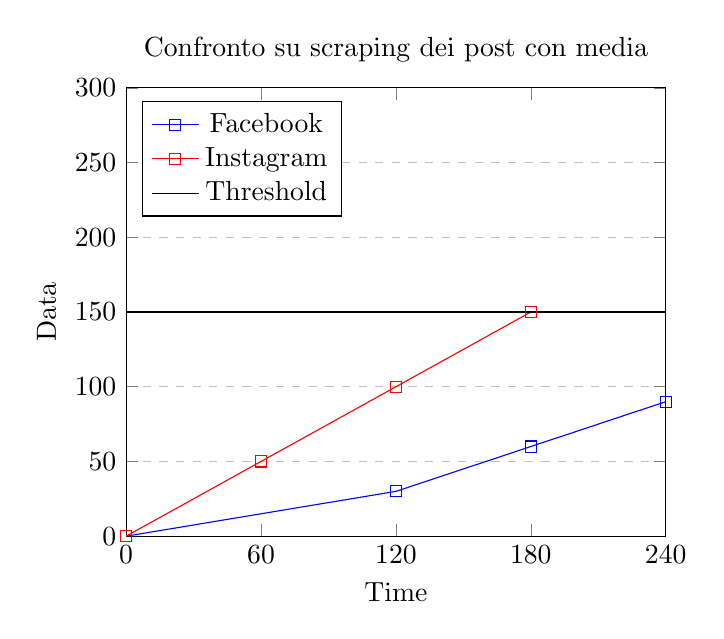
\begin{tikzpicture}
\begin{axis}[
    title={Confronto su scraping dei post con media},
    xlabel={Time},
    ylabel={Data},
    xmin=0, xmax=240,
    ymin=0, ymax=300,
    xtick={0,60,120,180,240},
    ytick={0,50,100,150,200,250,300},
    legend pos=north west,
    ymajorgrids=true,
    grid style=dashed,
]

\addplot[
    color=blue,
    mark=square,
    ]
    coordinates {
    (0,0)(120,30)(180,60)(240,90)
    };
    \legend{Facebook}
\addplot[
    color=red,
    mark=square,
    ]
    coordinates {
    (0,0)(60,50)(120,100)(180,150)
    };
\addplot[mark=none, black,samples=2] coordinates {(0,150)(240,150)};
    \legend{Facebook, Instagram, Threshold}
\end{axis}
\end{tikzpicture}
\end{center}
La soglia impostata equivale a 150 post.

Nel caso in cui venga raggiunta la soglia si procede con l'interruzione del servizio e l'avvio della funzione cookie o account rotation.

La media dello spazio di memoria occupato da una memorizzazione di 100 post (con foto e metadati in JSON) \`e di 100 Mb.
\begin{center}
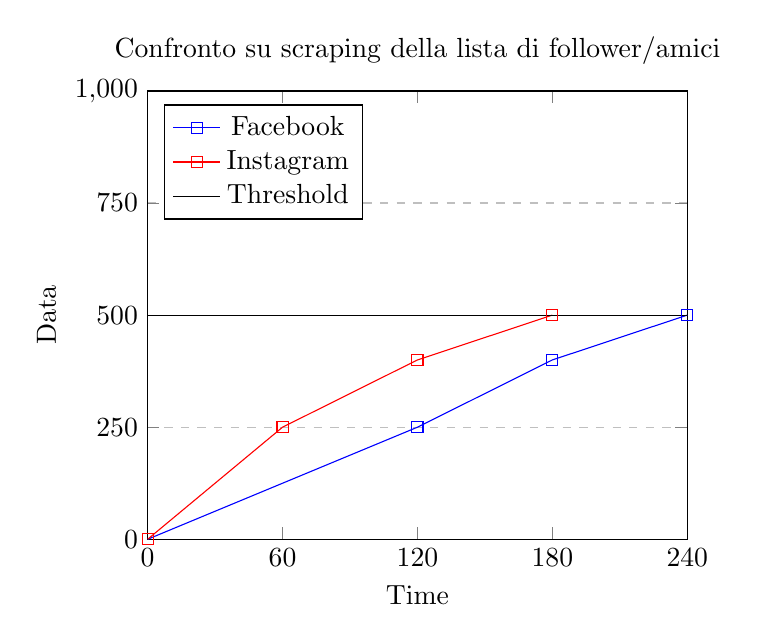
\begin{tikzpicture}
\begin{axis}[
    title={Confronto su scraping della lista di follower/amici},
    xlabel={Time},
    ylabel={Data},
    xmin=0, xmax=240,
    ymin=0, ymax=1000,
    xtick={0,60,120,180,240},
    ytick={0,250,500,750,1000},
    legend pos=north west,
    ymajorgrids=true,
    grid style=dashed,
]

\addplot[
    color=blue,
    mark=square,
    ]
    coordinates {
    (0,0)(120,250)(180,400)(240,500)
    };
    \legend{Facebook}
\addplot[
    color=red,
    mark=square,
    ]
    coordinates {
    (0,0)(60,250)(120,400)(180,500)
    };
\addplot[mark=none, black,samples=2] coordinates {(0,500)(240,500)};
    \legend{Facebook, Instagram, Threshold}
\end{axis}
\end{tikzpicture}
\end{center}
La soglia impostata equivale a 500 follower/amici.

Anche in questo caso, una volta raggiunta la soglia si interrompe il servizio per poi riprenderlo a seguito della rotazione degli account.

La liste prodotte in output sono dei file JSON e la loro occupazione di memoria dipende direttamente dalla quantit\`a di dati memorizzati. Il file JSON pu\`o arrivare ad occupare al massimo pochi Mb di spazio su disco.





\subsection{Osservazioni}
Il confronto dei connettori mette in luce come lo scraping di Instagram sia circa il doppio pi\`u veloce rispetto a quello di Facebook.
La motivazione risiede nella gestione dei dati e nella quantit\`a di informazioni aggregate ad un singolo post o ad una singola richiesta al server.

I principali problemi riscontrati nell'operativit\`a del software sono causati dalle soluzioni anti-scraping.

In particolare, da quanto osservato, il fulcro del contrasto avviene tramite l'analisi delle richieste, del numero di elementi estratti e dall'account utilizzato.

